%%%%%%%%%%%%%%%%%%%%%%%%%%%%%%%%%%%%%%%%%%%%%%%%%%%%%%%%%%%%%%%%%%%%%%%%%%%%%%%
% LAK27 Research Track submission -- JLA format
% Anonymized for double-blind review.
%%%%%%%%%%%%%%%%%%%%%%%%%%%%%%%%%%%%%%%%%%%%%%%%%%%%%%%%%%%%%%%%%%%%%%%%%%%%%%%

\documentclass[fleqn,10pt]{JLA_article}

\usepackage[english]{babel}
\usepackage{amsmath}
\usepackage{float}
\usepackage{array}

\usepackage{hyperref}
\hypersetup{hidelinks,colorlinks,breaklinks=true,urlcolor=color2,citecolor=color1,linkcolor=color1,bookmarksopen=false,pdftitle={Validity-Informed Attenuation},pdfauthor={Anonymous}}

%----------------------------------------------------------------------------------------
%	CITATION STYLE
%----------------------------------------------------------------------------------------
%
% apacite follows APA 6th, which spells out every author on the FIRST in-text
% citation of a 3-5 author work and only abbreviates to "et al." afterwards.
% APA 7th -- and the source manuscript's own usage -- abbreviates from the
% first citation onward.
%
% apacite provides \shortcite / \shortciteA, which always emit the abbreviated
% ("et al.") author list. Aliasing \cite and \citeA to them applies APA 7th
% behaviour document-wide, so no per-key bookkeeping is needed as references
% are added. Two-author and single-author works are unaffected: their
% abbreviated form is identical to their full form. The reference list itself
% is untouched and still lists all authors.
%
% To revert to apacite's default APA 6th behaviour, delete the two \let lines
% below. apacite's own \fullcite / \fullciteA are left intact and remain
% available if a spelled-out author list is ever wanted for a single citation.
\let\cite\shortcite
\let\citeA\shortciteA

%----------------------------------------------------------------------------------------
%	DRAFTING MARKERS -- REMOVE BEFORE SUBMISSION
%----------------------------------------------------------------------------------------

\newcommand{\todo}[1]{\textcolor{red}{\textbf{[TODO: #1]}}}
\newcommand{\citeneeded}[1]{\textcolor{red}{[cite: #1]}}

% \new marks text that is NOT verbatim from the source manuscript -- either
% written by me or reworded from the source. Black text is verbatim; red is not.
\newcommand{\new}[1]{\textcolor{red}{#1}}
\newenvironment{newcontent}{\color{red}}{\normalcolor}
%----------------------------------------------------------------------------------------
%	ARTICLE INFORMATION
%----------------------------------------------------------------------------------------

% TITLE NEEDS TO BE CHANGED
\PaperTitle{Validity-Informed Attenuation in Open-Ended Teaching Feedback: An Auditable Framework for Rating Sensitivity}

\Authors{Anonymous Author(s)}
\affiliation{\textsuperscript{1}\textit{Author affiliation withheld for double-blind review.}}

\Keywords{learning analytics; teaching feedback; validity; construct-irrelevant variance; aspect-based sentiment analysis; interpretability}

\Submitted{--/--/--}
\Accepted{--/--/--}
\Published{--/--/--}

\Volume{--}
\Number{--}
\Pages{1---14}
\Doi{xxx-xxx-xxx}

%----------------------------------------------------------------------------------------
%	NOTES FOR PRACTICE  --  required JLA element
%-------------------------  ---------------------------------------------------------------
\Notesname{Notes for Practice}

\note{\textbf{Users:} instructors and teaching/learning support staff interpreting open feedback.}

\note{\textbf{Use:} inspect a review's original text, topics, and adjustment trail; use it to distinguish potentially actionable pedagogical feedback from other student experience signals.}

\note{\textbf{Do not use:} automated ranking, promotion, tenure, discipline, or any high-stakes judgment about an instructor.}

\note{\textbf{Interpretation:} an attenuated value is a model-based alternative view under a stated relevance taxonomy; it is not a validated estimate of teaching quality.}

%----------------------------------------------------------------------------------------
%	ABSTRACT
%----------------------------------------------------------------------------------------

\Abstract{Open-ended teaching feedback combines pedagogical concerns with other expressions of student experience, yet numerical ratings collapse these signals into a single score. Existing computational approaches describe topics and sentiment but provide limited means to examine how an explicit relevance taxonomy shapes rating interpretation. Motivated by validity theory and robust-estimation principles, we introduce validity-informed attenuation, an auditable aspect-based sentiment analysis framework for examining rating sensitivity. The method attenuates emotion features from clauses assigned outside a stated pedagogical taxonomy in proportion to their share of review text, then records the resulting prediction change in a fixed rating model. Original reviews and the classification and adjustment trail remain available for inspection. We characterize the framework using 17,127 RateMyProfessors reviews, instructor-grouped model evaluation, and perturbation analyses. On held-out instructors, attenuation weakened associations between adjusted ratings and taxonomy-excluded emotion features while maintaining or slightly strengthening associations with included features. Three senior faculty experts judged 77 sampled review pairs. Ordering reviews by adjustment magnitude yielded 83.1\% agreement with expert majority judgments of validity and/or topical relevance, identical to the aggregate agreement of a density-only baseline. For both methods, agreement was higher on pairs with large adjustment contrasts than on those with smaller contrasts (100\% versus 61.8\%). Overall attenuation agreement exceeded a density-permutation benchmark, but agreement on smaller-contrast pairs did not. These findings provide an auditable mechanism and an initial evaluation reference for teaching-feedback analytics; improved teaching-quality measurement and benefits for stakeholder interpretation remain untested.}

%----------------------------------------------------------------------------------------

\begin{document}

\flushbottom
\maketitle
\thispagestyle{fancy}

%========================================================================================
\section{Introduction}
\addcontentsline{toc}{section}{Introduction}
%========================================================================================

\subsection{Open-Ended Teaching Feedback as a Learning-Analytics Trace}

Open-ended teaching feedback often pairs a single numerical rating with a comment spanning multiple topics of differing relevance to the intended evaluation. As a learning-analytics data source, this feedback offers context for examining numerical evaluations, but the rating alone does not reveal how these topics relate to the overall judgment. We argue that analytic approaches using these distinctions to reshape a rating summary require cautious interpretation, with relevance criteria and their effects made explicit and open to scrutiny.
The stakes of interpreting teaching feedback are particularly clear in Student Evaluations of Teaching (SET), where ratings are used as evidence in judgments about the quality of instruction. SET has historically guided consequential administrative decisions, raising concerns about how evaluations are interpreted and used in faculty assessment \cite{Haskell1997,Simpson2000,Irons2011,Wongsurawat2011,Zumbach2014,Emery2003,Dowell1983}. Despite this widespread usage, the validity of interpretations drawn from SET ratings remains contested: ratings may reflect influences beyond the instructional dimensions intended for evaluation \cite{Langbein1994,MarshRoche1997}. Situational factors, irrelevant content, and affective content unrelated to instruction threaten validity \cite{Wongsurawat2011,Schiekirka2015}, especially in informal instruments such as RateMyProfessors.com (RMP), which are fully open-ended, anonymized, and largely unmoderated. These concerns motivate making explicit which dimensions of student experience an analysis treats as relevant and how that choice shapes the resulting rating summary.

\subsection{The Unresolved Methodological Gap}

Existing computational SET research characterizes sentiment and topics, and predicts ratings, but offers few mechanisms connecting an explicit relevance taxonomy to model-estimated rating adjustments. We introduce \textbf{validity-informed attenuation}, an aspect-based sentiment analysis (ABSA) framework that scales emotion features from clauses assigned outside a stated relevance taxonomy---termed \emph{taxonomy-excluded affect}---and traces the resulting changes in a fitted rating model's predictions. Exclusion does not imply that the content is unimportant or invalid. The method makes rating sensitivity to the taxonomy auditable by preserving original reviews alongside classifications, emotion features, density values, and adjustment records. This supports a proposed human-review workflow where important criteria cannot be fully specified \cite{DoshiVelez2017} and analytics must connect to pedagogical interpretation and action \cite{GasevicDawsonSiemens2015}. Such inspectability makes the classification and adjustment process available for scrutiny, although the underlying predictive models retain black-box components \cite{Rybinski2021,Zhuang2025}.

\textbf{Research Questions:}

\begin{description}[noitemsep]
\item[RQ1.] What is the topic and affective composition of open-ended teaching feedback, and how do topic-specific emotional signals relate to numerical ratings in the fitted model?
\item[RQ2.] How does validity-informed attenuation change fitted-model outputs and feature associations on held-out instructors, and how stable are these changes under the tested perturbations?
\item[RQ3.] How do adjustment-magnitude and density-only orderings compare in their agreement with experts' relative judgments of review validity and/or topical relevance on sampled review pairs?
\end{description}

To answer our research questions, we develop and apply a five-stage NLP framework to 17,127 RMP student evaluations.

\subsection{Contributions}

\noindent The primary contributions of this research are:
\begin{itemize}
\item To our knowledge, the first auditable attenuation mechanism linking an explicit relevance taxonomy to traceable review-level adjustment records in a fitted rating model, motivated by validity and the down-weighting principle of robust estimation \cite{Messick1995,Huber1964}.
\item A proof-of-concept characterization of the mechanism on 17,127 RMP reviews, including held-out-instructor analyses and sensitivity checks.
\item An initial expert-comparison protocol and density-only reference results that assess agreement with expert rankings on sampled review pairs and establish a concrete baseline for future methods.
\end{itemize}

%========================================================================================
\section{Background and Conceptual Framing}
%========================================================================================

\subsection{Validity, Construct-Irrelevant Variance, and Teaching Feedback}

\citeA{Messick1995} identifies two primary threats to validity: construct underrepresentation and construct-irrelevant variance (CIV). His unified theory extends to any assessment in which responses are summarized into scores, a formulation that directly encompasses SET, with these threats particularly pronounced in informal, anonymous instruments such as RMP.

Both threats matter when defining a relevance taxonomy for teaching feedback: including extraneous content may introduce construct-irrelevant variance, while excluding relevant dimensions may underrepresent the intended construct. The taxonomy therefore operationalizes a relevance judgment whose coverage must itself remain open to scrutiny.

\citeA{MarshRoche1997} conclude that SET can be multidimensional, reliable, and relatively valid, but condition this on the content and coverage of items: ``scores averaged across an ill-defined assortment of items offer no basis for knowing what is being measured'' (p.\ 1187). Validity concerns the evidence supporting score interpretations and uses; the relevance and coverage of elicited content are part of that evidence \cite{Messick1995}. Unconstrained, open-ended instruments offer no design guarantee that responses adequately represent the intended construct.

\citeA{Wongsurawat2011} identifies pedagogically irrelevant comment content as a potential source of measurement error in open-ended SET and argues for evaluating comment reliability. Wongsurawat further argues that comments with little to no correlation with average evaluations should be discounted and that administrators would benefit from metrics quantifying comment quality and reliability.

Across these studies, validity threats from construct-irrelevant content, including situational confounders \cite{Schiekirka2015} and students' emotional and relational states \cite{Li2025}, are documented in both formal and informal evaluation contexts. Recent psychometric work has demonstrated that CIV can be identified and mitigated in constructed-response assessments under controlled conditions \cite{Zhai2021}, but applying this aim to open-ended teaching feedback requires an explicit basis for judging content relevance and examining how ratings respond when that relevance judgment is operationalized.

\subsection{From Descriptive NLP to Validity-Oriented Interpretation}

Prior SET research shows that aggregate sentiment can be associated with numerical ratings
\cite{Kechaou2011,Rajput2016,Iatrellis2024,Mihai2024}, but aggregation obscures topic-specific emotional context.
Deep-learning and ABSA (Aspect-Based Sentiment Analysis) techniques enable finer-grained representations of review
content \cite{Rybinski2021,Shuqin2024}; in SET, aspect-based approaches use this granularity to segment feedback and
extract aspect-level sentiment \cite{Bhowmik2023,Nikolic2020,Jazuli2025}. \citeA{Ren2022} extract and aggregate aspect
sentiment, while \citeA{Butt2025} compare BERT and LLM approaches for SET analysis.

Research on computational estimation of comment relevance shows that filtering by pedagogical value can improve prediction accuracy \cite{Sorour2015,Louis2013,Xiong2011}. These approaches leave open how an explicit relevance criterion can be connected to an auditable analysis of rating sensitivity.

\subsection{Design Principle: Attenuation Rather Than Deletion}

A review may contain both content relevant to the intended evaluation and content outside its scope, motivating a selective approach that retains the original feedback without excluding reviews. Robust estimation motivates down-weighting observations to limit their influence on an estimate \cite{Huber1964}. We adapt this general principle to topic-specific emotion features, using content density to determine the degree of attenuation.

Pedagogical relevance is operationalized through a generic three-category
taxonomy. Clauses assigned to \textit{Miscellaneous} fall outside the included
dimensions; because this residual category may include omitted pedagogical
concerns, ambiguous wording, or classification error, it provides a basis for
inspection rather than a determination of irrelevance. The three categories
reflect dimensions that recur across SET instruments and research syntheses
\cite{Marsh1982}, chosen as a generic, widely legible baseline; different taxonomies would produce different
density estimates and adjustments. If further refinement and validation support application to formal SET, stakeholders could
define or refine the categories in relation to course learning design and its
documented pedagogical intent, so that the analytic lens reflects local priorities
\cite{LockyerHeathcoteDawson2013}.

These considerations motivate a proof of concept connecting an explicit relevance taxonomy to an auditable analysis of rating sensitivity, with outputs open to scrutiny and contestation \cite{DrachslerGreller2016} and intended to support pedagogical interpretation and action \cite{GasevicDawsonSiemens2015}.
%========================================================================================
\section{Method}
%========================================================================================

\subsection{Study Context and Data}

RMP provides a noisy setting for examining heterogeneous and idiosyncratic, informal teaching feedback rather than a proxy for institutional SET. Because RMP prohibits scraping and our requests for permission to collect data directly were unsuccessful, we use the existing dataset provided by \citeA{He2020}. It contains more than 19,000 reviews with numerical ratings (1--5) for hundreds of professors. We do not use its RMP meta-tags or demographic information.

We excluded non-English reviews, reviews containing RMP's automatic censorship string ``****'' (whose application was prone to error), entries with no review text or text such as ``No Comment'', and reviews for professors with fewer than eight total reviews. After these exclusions, the final dataset contains 17,127 reviews. Reviews were then cleaned (encoding repair via \texttt{ftfy}, lowercase normalization, abbreviation expansion, and punctuation standardization); stemming and lemmatization were withheld to preserve contextual information for downstream models.

\subsection{Aspect-Term Categorization}

Cleaned text is separated into individual clauses using \texttt{spaCy}'s \texttt{en\_core\_web\_sm} model, which segments text based on punctuation while attempting to avoid splits on non-statement punctuation. When punctuation is sparse, two additional rules split text on commas and stop-words (but, so, yet), with aggressive stop-word separation used for reviews containing no punctuation.

The next stage assigns each review clause to one of three categories included in this study’s pedagogical interpretation---\textit{Instructional Effectiveness}, \textit{Fairness \& Grading}, and \textit{Workload \& Difficulty}---or to \textit{Miscellaneous}, a residual category for clauses not assigned to those dimensions. Each pedagogical topic is defined using multiple short natural-language descriptions of common student expressions. These descriptions and each review clause are encoded using the pretrained sentence-embedding model \texttt{all-mpnet-base-v2}. Each category representation is the elementwise mean of its descriptor
embeddings; clause assignment uses cosine similarity against that mean and the clause is assigned as follows:

\begin{equation}
\text{topic}(c) =
\begin{cases}
\displaystyle \arg\max_{k \in \{\text{eff},\,\text{fair},\,\text{work}\}} s_{c,k}, & \text{if } \max_{k \in \{\text{eff},\,\text{fair},\,\text{work}\}} s_{c,k} > \tau, \\
\textit{Miscellaneous}, & \text{otherwise},
\end{cases}
\end{equation}
where $s_{c,k}$ represents the cosine similarity between clause $c$ and pedagogical topic $k$. We set $\tau=0.25$ selected on a development set of 386 clauses from 100 manually inspected reviews, drawn before and independently of the evaluation
sample, which was matched in size; the two samples share a single review, whose
ten clauses appear in both. Threshold selection was thus out-of-sample except
for these ten clauses (2.6\% of the evaluation sample).

Table~\ref{tab:atc-taxonomy} summarises the four-category taxonomy with representative descriptor phrases used to construct each topic embedding.

\begin{table}[htbp]
\caption{Aspect-term categorization taxonomy and representative descriptor phrases.}
\label{tab:atc-taxonomy}
\centering
\small
\begin{tabular}{p{3.8cm}p{8.2cm}}
\toprule
\textbf{Category} & \textbf{Representative Descriptors} \\
\midrule
Instructional Effectiveness & Clear and effective explanations of concepts; lectures are well-organized and easy to follow; helps students learn \\
\addlinespace
Fairness \& Grading & Grading feels fair, earned, and based on actual performance; tough but fair grader; adjusts grading to student's current ability \\
\addlinespace
Workload \& Difficulty & Heavy workload, lots of effort and time required; tests, exams, or quizzes are hard or demanding; easy class, light workload \\
\addlinespace
Miscellaneous & Clauses below the similarity threshold $\tau$ for all pedagogical categories; includes personal remarks and social commentary \\
\end{tabular}
\end{table}

\subsection{Pedagogical Density and Per-Clause Emotion Extraction}

Using the categorized statements, density metrics are calculated for each review:
\begin{equation}
D_{\text{misc}} =
\frac{\text{wordcount}_{\text{misc}}}
{\text{total wordcount}},
\qquad
D_{k} =
\frac{\text{wordcount}_{k}}
{1 + \text{wordcount}_{k} + \text{wordcount}_{\text{misc}}},
\quad k \in \{\text{eff},\,\text{fair},\,\text{work}\}.
\end{equation}

Here, $D_{\text{misc}}$ is the proportion of review words assigned to \textit{Miscellaneous}, and $1-D_{\text{misc}}$ is the proportion assigned to included categories; neither establishes individual clauses' pedagogical relevance. The added one in $D_k$ prevents division by zero when both topic $k$ and \textit{Miscellaneous} are absent. The pedagogical densities $D_k$ serve as regression predictors but do not determine attenuation.

Per-clause sentiment analysis is performed using \texttt{SamLowe/roberta-base-go\_emotions} \cite{sam_lowe_2024}, a fine-tuned RoBERTa model trained on the GoEmotions dataset \cite{Demszky2020}. Each clause $c$ is independently processed and represented by a 27-dimensional emotion vector $\mathbf{e}'_c$, where each component denotes the probability estimated by the model that the clause expresses an emotion label. The model initially produces the 28 GoEmotions labels; \textit{Neutral} is removed because it simply represents the absence of strong emotional activation.

  For each review, we average clause-level emotion vectors within each topic $k$:

\begin{equation}
\mathbf{E}_k = \frac{1}{|C_k|} \sum_{c \in C_k} \mathbf{e}'_c,
\end{equation}

where $C_k$ is the set of review clauses assigned to topic $k$. If $C_k$ is empty, $\mathbf{E}_k$ is a 27-dimensional zero vector, preserving the input dimensionality.

\subsection{Predicting Ratings from Topic Specific Emotions}

Ratings are modelled as a function of emotions directed towards each topic and density metrics. For a single review, the input feature vector is represented as:

\begin{equation}
\mathbf{x}_{\text{review}} =
\Big[
\begin{aligned}
&\mathbf{E}_{\text{eff}}, \;\mathbf{E}_{\text{fair}}, \;\mathbf{E}_{\text{work}}, \;\mathbf{E}_{\text{misc}},\\
& D_{\text{eff}}, \; D_{\text{fair}}, \; D_{\text{work}}, \; D_{\text{misc}}
\end{aligned}
\Big]
\in \mathbb{R}^{4 \times 27 + 4} = \mathbb{R}^{112}.
\end{equation}

For $N=17{,}127$ reviews, the feature matrix is $\mathbf{X} \in \mathbb{R}^{N \times 112}$.

To prevent instructor overlap between training and evaluation and assess generalization to unseen professors, we use an 80--20 professor-level split: 823 training and 206 held-out professors. Model-performance and coherence analyses use held-out professors; the curated expert-comparison sample spans both groups.

We employ CatBoost regression, an open-source gradient-boosted tree model that captures non-linear interactions between emotional signals and topics in the sparse review representation \cite{Hancock2020,Prokhorenkova2018,Dorogush2018}. The final configuration was selected through grouped 5-fold cross-validation (GroupKFold, grouped by professor ID) on the training professors: 1000 iterations, learning rate 0.02, depth 7, and L2 leaf regularization 6; all other hyperparameters were kept at their default values. MAE was used as both the loss function and evaluation metric because it measures average absolute deviation from ratings on the 1--5 scale and is resilient to occasional outliers.

\subsection{Validity-Informed Attenuation \& Rating Adjustment}

Density measures the proportion of taxonomy-excluded text; the attenuation-based rating adjustment measures the fitted
model's response to a density-dependent perturbation of \textit{Miscellaneous} emotion features. We calculate the
down-weighting factor $\zeta$ as:

\begin{equation}
    \zeta = 1-D_{\text{misc}}.
\end{equation}

When $D_{\text{misc}}=0$, the review is unchanged ($\zeta=1$); when $D_{\text{misc}}=1$, its \textit{Miscellaneous} emotion features are zeroed ($\zeta=0$). Intermediate densities produce proportional attenuation:

\begin{equation}
    \hat{E}_{\text{misc}}^{\text{weighted}} = E_{\text{misc}} \cdot \zeta.
\end{equation}

Applying the trained CatBoost model $f_\mathrm{CB}$, held fixed across conditions, to the baseline and attenuated feature vectors produces:

\begin{equation}
\begin{aligned}
\hat{y}_i^\text{attenuated} &= f_\mathrm{CB}\big(\hat{\mathbf{x}}_i^\text{weighted}\big), \\
\hat{y}_i^\text{baseline} &= f_\mathrm{CB}(\mathbf{x}_i), \qquad i = 1, \dots, N.
\end{aligned}
\end{equation}

Adjusted ratings are defined as:

\begin{equation}
\hat{y}_i^\text{adjusted} = y_i^\text{raw} + \big( \hat{y}_i^\text{attenuated} - \hat{y}_i^\text{baseline}\big), \quad i = 1, \dots, N.
\end{equation}

The prediction difference $\Delta_i = \hat{y}_i^\text{attenuated} - \hat{y}_i^\text{baseline}$ quantifies the fitted
  model's response to scaling the \textit{Miscellaneous} emotion features. All other input features remain fixed, while
  the prediction difference reflects the model's learned relationships and interactions. Adding $\Delta_i$ to the raw
  rating preserves the original prediction residual and yields a model-based alternative summary under the stated
  attenuation rule.

Because attenuation evaluates the fitted model at transformed feature
configurations, its outputs characterize the model's response to the specified
transformation rather than ratings that would have been empirically observed.
Most sharply, at $D_{\text{misc}}=1$ all emotion features are zero and every such
review receives an identical attenuated prediction, a property of the
representation and fitted model rather than an empirically validated
affect-neutral target.

\subsubsection{Audit Trail and Worked Example}

Table~\ref{tab:ex2} presents an end-to-end trace of an individual review with high \textit{Miscellaneous} density ($D_{\text{misc}}$=0.670), where affect in the \textit{Miscellaneous} category dominates, receiving a positive adjustment of $+$0.427. The trace also makes contestable assignments visible for review: under this generic taxonomy, the classifier assigns interpersonal-conduct language to \textit{Miscellaneous} and subject-knowledge language to \textit{Instructional Effectiveness}. 

\begin{table}[htbp]
    \caption{Worked Example, Review \#14848.}
    \label{tab:ex2}
    \centering
    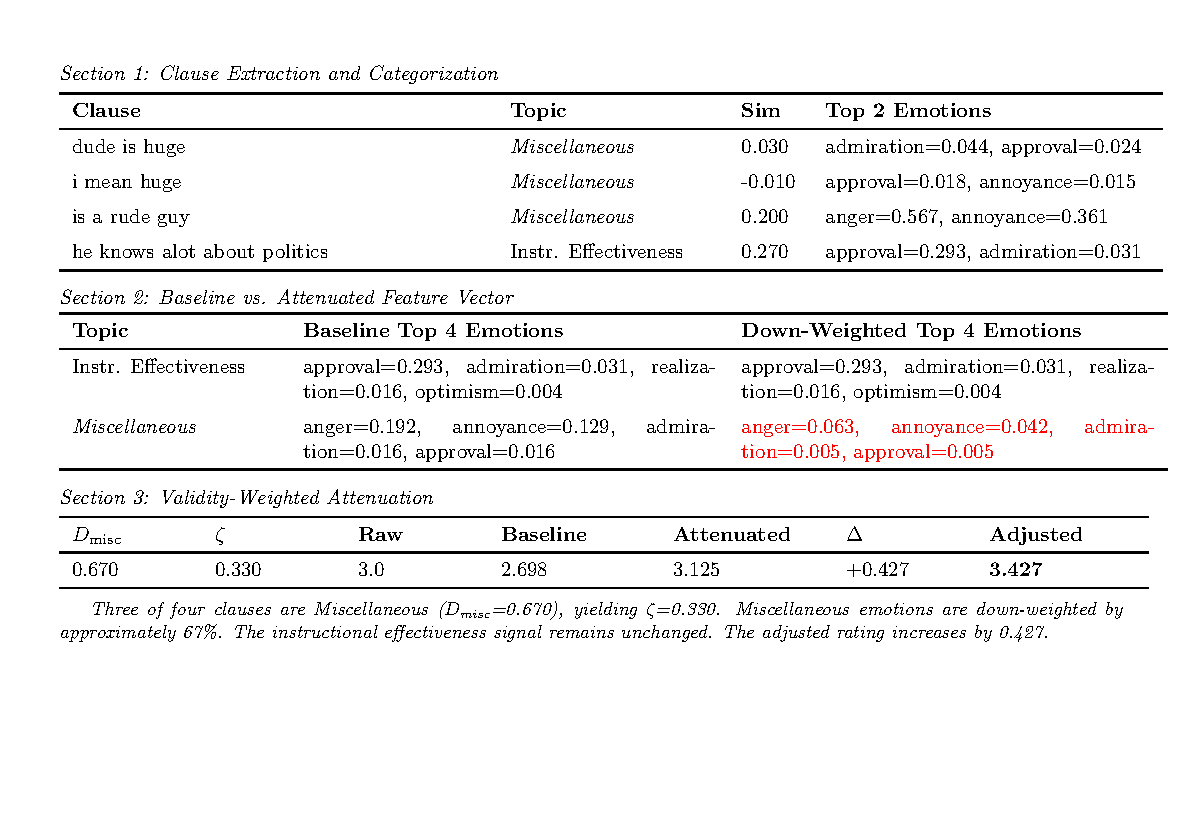
\includegraphics[trim=10 89 15 43, clip, width=\linewidth]{Diagrams/pdfs/ex2.pdf}
\end{table}

%========================================================================================
\section{Results}
%========================================================================================

\subsection{Corpus and Model Behaviour}

\subsubsection{ATC Topic Structure}

Table~\ref{tab:clause_review_freq} summarises topic frequencies after ATC. \textit{Instructional Effectiveness} is the most frequent topic at both clause and review level, followed by \textit{Miscellaneous} and \textit{Workload}, with \textit{Fairness} trailing substantially. The prominence of \textit{Miscellaneous} clauses indicates that a substantial portion of student discourse falls outside this study's included pedagogical dimensions.

The rating distribution is negatively skewed, yet low-rating reviews show distinctive patterns: for ratings 1.0--2.0, \textit{Miscellaneous} clauses are the most frequent topic, exceeding the next pedagogical category by approximately 27\% in 1-star reviews.


Across all reviews, $D_{\text{misc}}$ is heavily right-skewed (median 0.11, mean 0.22), with a spike at $D_{\text{misc}}=1$ representing wholly \textit{Miscellaneous} reviews receiving maximal attenuation (Figure~\ref{fig:dmisc_dist}).

\begin{table}[htbp]
\centering
\caption{Clause and review-level topic frequencies.}
\label{tab:clause_review_freq}
\small
\begin{tabular}{lccc}
\toprule
\textbf{Topic} & \textbf{Clause} & \textbf{Review} & \textbf{Avg./Review} \\
\midrule
\textit{Instructional Eff.} & 25,845 & 13,494 & \textbf{1.92} \\
\textit{Miscellaneous} & 17,602 & 10,375 & \textbf{1.70} \\
\textit{Workload} & 15,683 & 9,387 & \textbf{1.67} \\
\textit{Fairness} & 4,258 & 3,567 & \textbf{1.19} \\
\bottomrule
\end{tabular}
\end{table}

\begin{figure}[htbp]
    \centering
    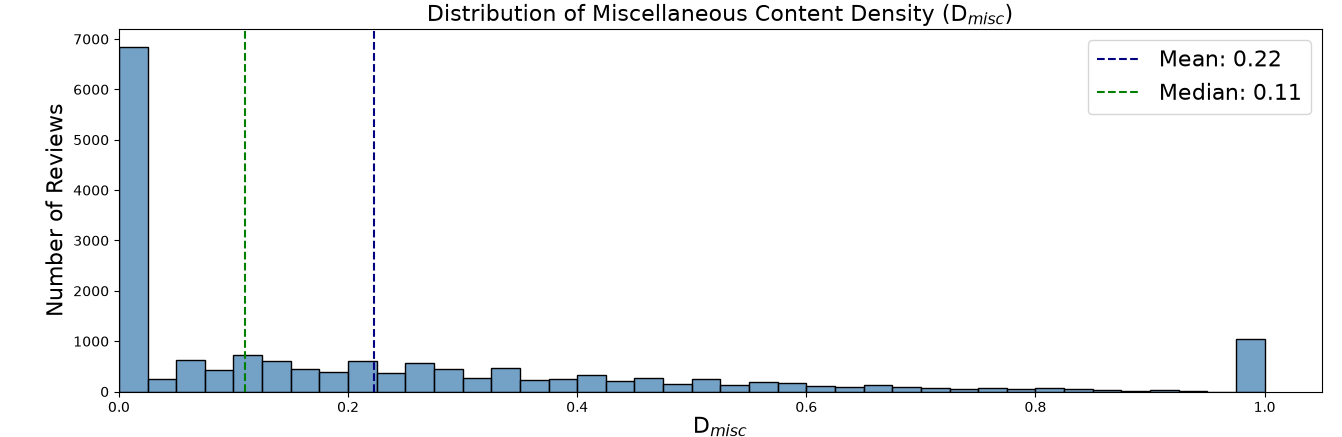
\includegraphics[width=0.72\linewidth]{Diagrams/atc_visuals/dmiscdistribution.png}
    \caption{$D_\text{misc}$ distribution across all reviews.}
    \label{fig:dmisc_dist}
\end{figure}

\subsubsection{Sentiment Extraction}

RoBERTa-GoEmotions outputs show higher positive-emotion label probabilities in high-rated reviews and higher negative-emotion label probabilities in low-rated reviews, with cross-valence signals at both extremes (Figure~\ref{fig:one-star-emotion-heatmap} illustrates one-star reviews). These outputs may reflect mixed emotional expression, sarcasm, or classification error.

\begin{figure}[htbp]
    \centering
    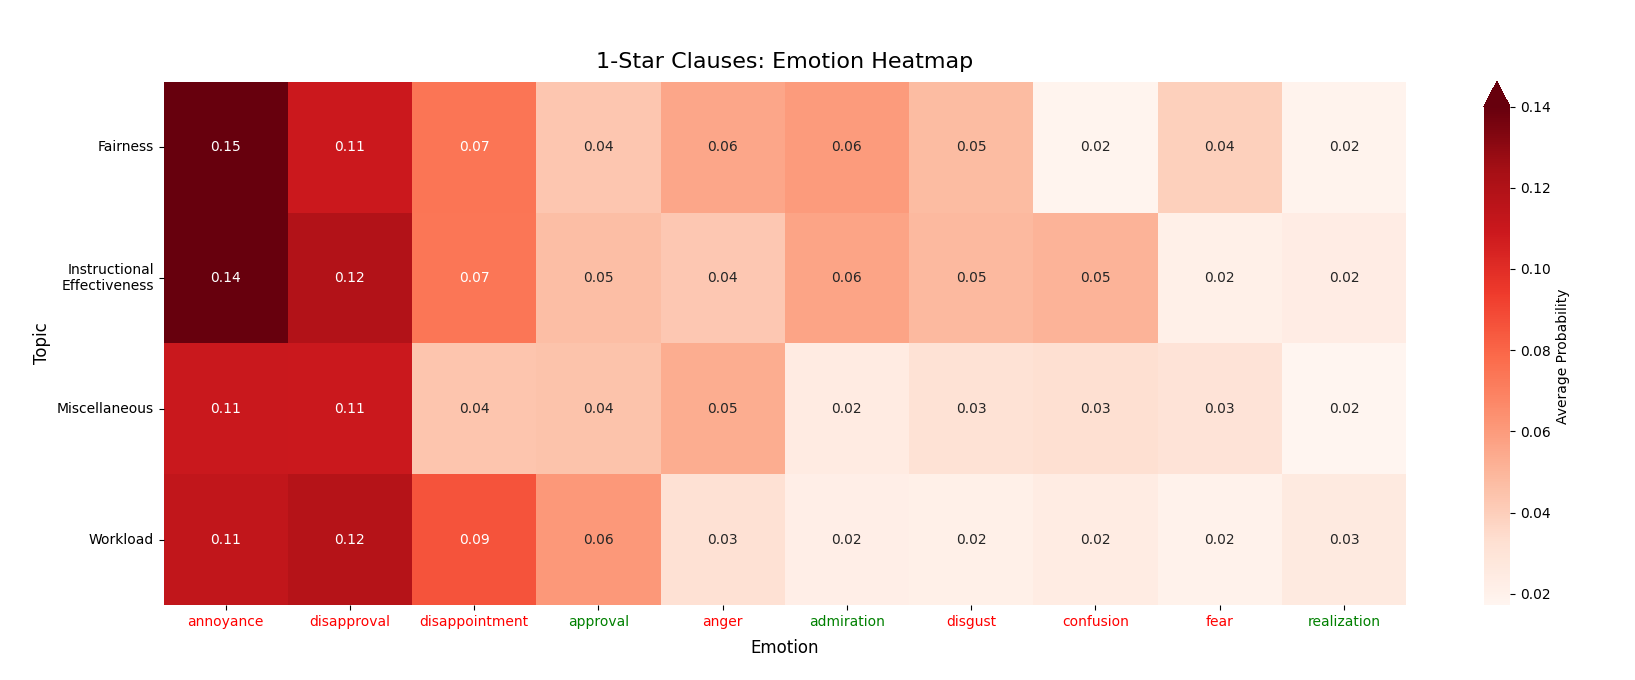
\includegraphics[width=\linewidth]{Diagrams/roberta/1_star_heatmap_emotions.png}
    \caption{Average emotion probabilities by topic for one-star clauses.}
    \label{fig:one-star-emotion-heatmap}
\end{figure}

\subsubsection{ATC Validation}

To characterize inter-model consistency in applying the taxonomy, two independent LLMs (GPT-5 mini and Grok 4.1)
categorized 386 clauses, yielding Cohen's \citeyear{Cohen1960} $\kappa = 0.7273$ (“substantial agreement”;
\citeNP{Landis1977}).

A senior faculty expert with more than 15 years of teaching and evaluation experience independently labelled the same 386 clauses, with multiple valid categories permitted per clause. Under a containment criterion (correct if the model's category appeared in the expert's label set), accuracy is 0.77. Restricting to clauses with exactly one expert label ($n = 287$) yields strict accuracy of 0.72; Table~\ref{tab:atc-classification-report} reports per-category precision, recall, and F1.

\begin{table}[htbp]
    \caption{Single-label classification performance of ATC against expert annotations.}
    \label{tab:atc-classification-report}

    \centering
    \begin{minipage}[t]{0.48\linewidth}
        \centering
        \small
        \begin{tabular*}{\linewidth}{@{\extracolsep{\fill}}lccccc@{}}
        \textbf{Category} & \textbf{Precision} & \textbf{Recall} & \textbf{F1} & \textbf{Support} \\
        \hline
        \textit{Instr. Eff.} & 0.73 & 0.76 & 0.74 & 99 \\
        \textit{Fairness} & 0.57 & 0.76 & 0.65 & 17 \\
        \textit{Workload} & 0.63 & 0.78 & 0.69 & 54 \\
        \textit{Miscellaneous} & 0.82 & 0.66 & 0.73 & 117 \\
        \hline
        \end{tabular*}
    \end{minipage}\hfill
    \begin{minipage}[t]{0.48\linewidth}
        \centering
        \small
        \begin{tabular*}{\linewidth}{@{\extracolsep{\fill}}lccccc@{}}
         & \textbf{Precision} & \textbf{Recall} & \textbf{F1} & \textbf{Support} \\
        \hline
        Macro Avg & 0.68 & 0.74 & 0.70 & 287 \\
        Weighted Avg & 0.74 & 0.72 & 0.72 & 287 \\
        \hline
        Accuracy & \multicolumn{4}{c}{0.72 (n = 287)} \\
        \hline
        \end{tabular*}
    \end{minipage}
\end{table}

These results indicate acceptable alignment for a proof-of-concept study, though accuracy leaves room for improvement, particularly for \textit{Fairness} and \textit{Workload} where support is limited.

\subsubsection{Rating Regression Performance}

Table~\ref{tab:model-performance} reports 5-fold GroupKFold CV and held-out performance; the held-out MAE of 0.6347 falls inside the fold range, suggesting consistent generalization.

\begin{table}[htbp]
\caption{CatBoost 5-fold CV and held-out performance.}
\label{tab:model-performance}
\centering
\small
\begin{tabular}{lccc}
\toprule
& MAE & Spearman $\rho$ & $R^2$ \\
\midrule
5-fold CV mean & 0.6300 & 0.7284 & 0.6255 \\
$\pm$SD & $\pm 0.0081$ & $\pm 0.0152$ & $\pm 0.0088$ \\
\midrule
Held-out professors & 0.6347 & 0.7352 & 0.6168 \\
\bottomrule
\end{tabular}
\end{table}

The final model demonstrates low absolute error, strong ordinal consistency, and substantial explained variance on held-out data, suggesting that it captures meaningful relationships between emotional content and student ratings.

SHAP values \cite{LundbergLee2017} were computed using exact TreeSHAP on
held-out reviews, relative to the model's expected value. For directional
inspection, per-review SHAP values were averaged within each of the eight
polarity--topic groups. Beeswarm results show broadly coherent directional patterns: higher positive-emotion feature values generally contribute positively to predicted ratings, while higher negative-emotion feature values generally contribute negatively. At lower feature values, these contribution patterns can reverse (Figure~\ref{fig:baseline-shap}).

\begin{figure*}[tbp]
    \centering
    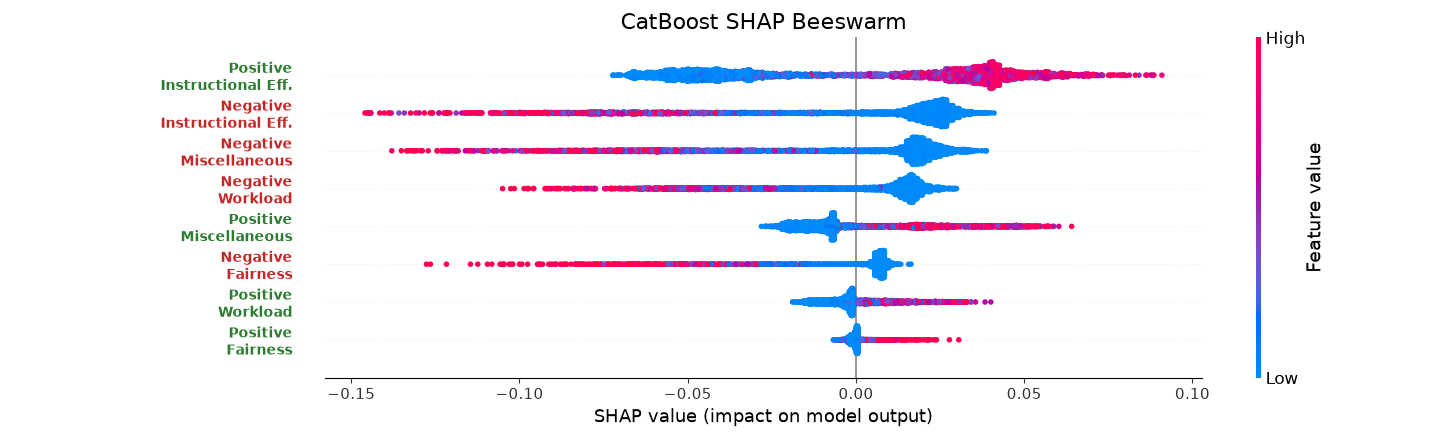
\includegraphics[width=0.90\textwidth]{Diagrams/SHAP/baseline_shap.png}
    \caption{SHAP beeswarm plot for the eight polarity $\times$ topic categories on held-out professors. Point colour indicates feature value; horizontal position shows each feature's contribution to the predicted rating.}
    \label{fig:baseline-shap}
\end{figure*}

\subsection{What Attenuation Changes}

We evaluate whether attenuation produces structured and interpretable changes, examining feature importance shifts, correlation changes, and the relationship between attenuation $\Delta$s and modulators ($D_{misc}$, $E_{misc}$).

\subsubsection{Adjustment Outcomes}

Of the 17,127 reviews, 10,375 (60.58\%) contained \textit{Miscellaneous} content. Within this subset, the mean $|\Delta|$ was 0.1964 and the mean signed $\Delta$ was 0.0440 (Wilcoxon signed-rank $W = 24{,}260{,}091$, $p < .001$); reviews cluster within
instructors, so the descriptive pattern rather than the significance level
carries the interpretation. The professor-level distribution shape remained largely consistent. Adjustments form a two-sided tail: individual values range from $-1.39$ to $+2.71$ rating points, with the largest magnitudes concentrated in reviews combining high taxonomy-excluded density with high miscellaneous emotion-label probabilities.

The analyses that follow use the 206 held-out professors: 3,414 reviews for feature-importance analyses and 2,052 reviews containing \textit{Miscellaneous} content for correlation and modulator analyses.

\subsubsection{Mechanistic Coherence}

Figure~\ref{fig:mechanistic-checks} and Table~\ref{tab:correlation_deltas} summarise three coherence checks on held-out professors.  Per-review absolute SHAP-based model contributions were summed within each topic group and averaged across reviews, with changes expressed relative to each group's baseline. Feature importance shifts away from \textit{Miscellaneous} sentiment and toward pedagogically relevant categories (Figure~\ref{fig:mechanistic-checks}a). Pearson and Spearman correlations between baseline emotion features and ratings show the same pattern: \textit{Miscellaneous} associations weaken while pedagogical associations are maintained or slightly strengthened (Figure~\ref{fig:mechanistic-checks}b). These comparisons use the same emotion features before and after attenuation; only the rating changes.

\begin{figure*}[tbp]
    \centering
    \begin{minipage}[t]{0.48\textwidth}
        \centering
        \textbf{(a)}\\[-0.25em]
        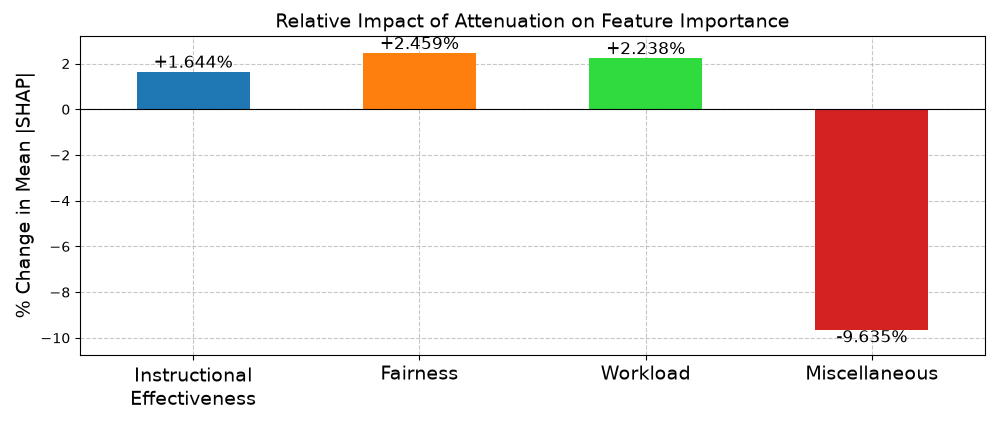
\includegraphics[width=\linewidth]{Diagrams/SHAP/pct_change_shap.png}
    \end{minipage}\hfill
    \begin{minipage}[t]{0.48\textwidth}
        \centering
        \textbf{(b)}\\[-0.25em]
        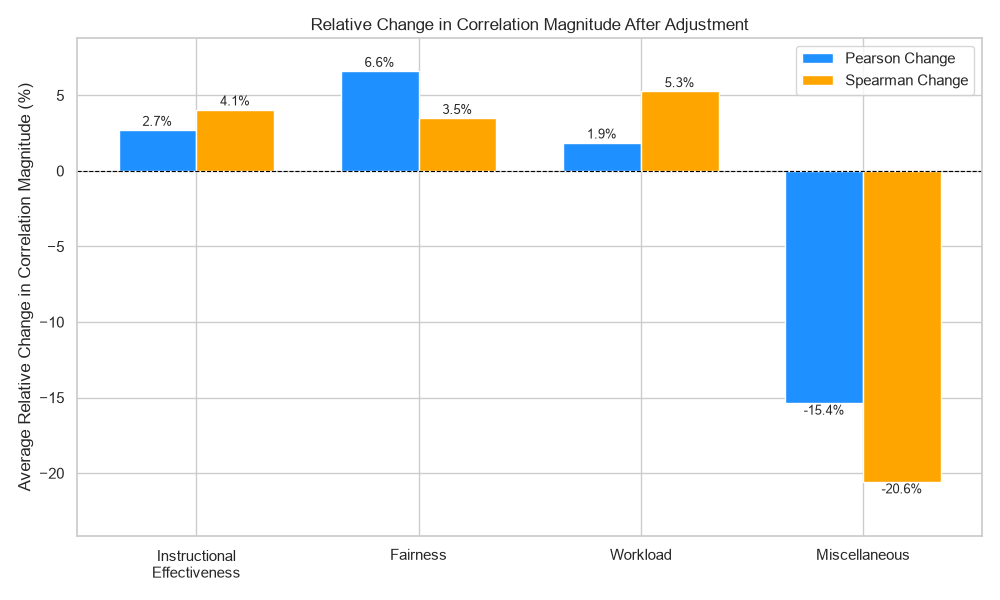
\includegraphics[width=\linewidth]{Diagrams/correlation_changes/average_corr_changes.png}
    \end{minipage}
    \caption{Mechanistic coherence checks after attenuation. (a) Change in SHAP-based feature importance (\%), computed on held-out professors ($n = 3{,}414$ reviews). (b) Average change in correlation magnitude (\%, Pearson and Spearman) after adjustment, held-out professors ($n = 2{,}052$). Bars show mean $(|\text{corr}_{\text{adjusted}}| - |\text{corr}_{\text{raw}}|)/|\text{corr}_{\text{raw}}|$ across polarity groups.}
    \label{fig:mechanistic-checks}
\end{figure*}


\begin{table}[htbp]
    \caption{Correlation analysis: attenuation $\Delta$ versus modulators, computed on held-out professors ($n = 2{,}052$ reviews).}
    \label{tab:correlation_deltas}
    \centering
    \begin{minipage}[t]{0.48\linewidth}
        \centering
        \small
        \textbf{(a) Density modulator $D_{\text{misc}}$}\\[0.2em]
        \begin{tabular*}{\linewidth}{@{\extracolsep{\fill}}lcc@{}}
        \toprule
        Relationship & Pearson $r$ & Spearman $\rho$ \\
        \midrule
        $\Delta^+$ vs. $D_{\text{misc}}$ & 0.6872 & 0.6142 \\
        $\Delta^-$ vs. $D_{\text{misc}}$ & $-$0.7077 & $-$0.6001 \\
        \bottomrule
        \end{tabular*}
    \end{minipage}\hfill
    \begin{minipage}[t]{0.48\linewidth}
        \centering
        \small
        \textbf{(b) Emotion-signal modulator $E_{\text{misc}}$}\\[0.2em]
        \begin{tabular*}{\linewidth}{@{\extracolsep{\fill}}lcc@{}}
        \toprule
        Relationship & Pearson $r$ & Spearman $\rho$ \\
        \midrule
        $\Delta^+$ vs. Neg. $E_{\text{misc}}$ & 0.4008 & 0.4327 \\
        $\Delta^-$ vs. Pos. $E_{\text{misc}}$ & $-$0.2470 & $-$0.1125 \\
        \bottomrule
        \end{tabular*}
    \end{minipage}
\end{table}

$D_{misc}$ is the primary driver of attenuation magnitude (Table~\ref{tab:correlation_deltas}a): adjustment magnitude increases with \textit{Miscellaneous} density, while correlations with miscellaneous emotion features are weaker but directionally consistent. A Mann-Whitney U test~\cite{MannWhitney1947} with rank-biserial effect size~\cite{Cureton1956} confirms significantly larger absolute adjustments for reviews with higher \textit{Miscellaneous} density ($D_{\text{misc}} > 0.5$, $n=508$) than for reviews with lower density ($D_{\text{misc}} < 0.2$, $n=690$) ($U = 313{,}494$, $p < .001$, $|r| = .789$).Reviews cluster within instructors, and some instructors appear in both
density groups, so the effect size rather than the significance level carries
the interpretation. Together, these checks indicate that attenuation introduces structured and interpretable adjustments consistent with its design rationale.

\subsection{Initial Validity and Robustness Evidence}

\subsubsection{Expert Paired Comparisons}

Three senior faculty experts with 75 combined years of teaching, evaluation, and supervision experience independently labelled the same 80 RMP review pairs. Experts were blind to model outputs and one another's labels; three pairs without model outputs were included to further blind them. Instructor and institution names were replaced with tags; profanity and emoji were replaced where present. Pair order was randomized once and shared across experts. Identical prompts asked experts to select the review that was ``more valid and/or on topic,'' or respond ``completely unsure.'' This single comparative judgment left validity and topical relevance to professional judgment, without separating them or supplying the study taxonomy. The verbatim prompt is provided in the supplementary material. Pairs were constructed by randomly sampling an initial review, informally checking its ATC assignment, and sampling a second review until the required adjustment-contrast bin was met. Candidate rejection counts during pair construction were not recorded. Excluding the three pairs without model outputs, there were 77 evaluable pairs: 43 coarse and 34 fine. Coarse pairs had an absolute-adjustment difference $\bigl||\Delta_1|-|\Delta_2|\bigr| \geq 0.5$; fine pairs had a difference below 0.5. At the operating point $s=1$, these conditions partition the evaluable pairs. The 77 pairs reference 144 distinct instructors; eight instructors appear in more than one pair (at most three), and no pair contains two reviews of the same instructor.

Two matching votes established a majority. A model ranking agreed when the review receiving smaller $|\Delta|$ matched a directional majority; exact model ties selected the first displayed review. Density alone selects the review with lower $D_{\text{misc}}$, with density ties counted as incorrect. This comparison tests whether ordering reviews by the magnitude of the fitted model's response to taxonomy-based attenuation aligns with experts' judgments of validity and/or topical relevance. All retained pairs had three votes and a majority; one ``unsure'' majority counted as incorrect. Table~\ref{tab:expert-consensus} reports majority agreement, two-sided 95\% Wilson \citeyear{Wilson1927} intervals, and Fleiss' \citeyear{Fleiss1971} $\kappa$ over all three response categories. Following \cite{Landis1977}, these correspond to substantial ($\kappa=.658$, overall), almost perfect ($\kappa=.819$, coarse), and moderate ($\kappa=.469$, fine) agreement. Individual-expert fine agreement ranged from 58.8\% to 70.6\%. Excluding individual non-directional votes raised fine inter-expert agreement to $\kappa=.634$ (``substantial agreement''); this does not change the primary scoring.

\begin{table}[htbp]
\centering
\small
\caption{Attenuation and density-only rankings compared with three-expert judgments on the same 77 pairs and original attenuation-defined coarse/fine groups.}
\label{tab:expert-consensus}
\begin{tabular}{lccccc}
\toprule
\textbf{Condition} & \shortstack{\textbf{Attenuation}\\\textbf{correct/$n$}} & \shortstack{\textbf{Density-only}\\\textbf{correct/$n$}} & \shortstack{\textbf{Agreement}\\\textbf{for each}} & \shortstack{\textbf{95\% CI}\\\textbf{for each}} & \textbf{Expert} $\boldsymbol{\kappa}$ \\
\midrule
Overall & 64/77 & 64/77 & 83.1\% & [73.2\%, 89.9\%] & .658 \\
Coarse  & 43/43 & 43/43 & 100\%  & [91.8\%, 100\%]  & .819 \\
Fine    & 21/34 & 21/34 & 61.8\% & [45.0\%, 76.1\%] & .469 \\
\bottomrule
\end{tabular}
\end{table}

A post hoc diagnostic partitioned the 34 fine pairs by expert voting pattern: of 19 unanimous pairs, 16 agreed with the model ranking (84.2\%); of 15 split-vote pairs, 5 agreed (33.3\%). Ten of thirteen model--majority disagreements occurred on pairs where the experts themselves disagreed. Three disagreements persisted despite expert unanimity, at absolute-adjustment contrasts of 0.314, 0.005, and 0.026 points.

Density alone matched attenuation's agreement overall and within both contrast groups. Both methods correctly ranked 61 pairs; each correctly ranked three additional pairs that the other did not. Thus, this sample shows no aggregate agreement advantage for attenuation over density alone. Table~\ref{tab:discordant} presents one exclusive success for each method.
\begin{table}[htbp]
\caption{Two discordant expert-comparison pairs illustrating differences between density-based and adjustment-magnitude ordering. Density selects the review with lower $D_{\text{misc}}$; attenuation selects the review with smaller $|\Delta|$. All six discordant pairs are provided in the supplementary material.}
\label{tab:discordant}
\small
\centering
\setlength{\tabcolsep}{4pt}
\renewcommand{\arraystretch}{1.1}
\begin{tabular}{>{\raggedright\arraybackslash}p{0.13\linewidth}>{\raggedright\arraybackslash}p{0.46\linewidth}>{\raggedright\arraybackslash}p{0.38\linewidth}}
\toprule
 & \shortstack[l]{\textbf{Pair 1}\\\textit{attenuation correct}} & \shortstack[l]{\textbf{Pair 6}\\\textit{density correct}} \\
\midrule
 $D_{\text{misc}}$ (Rev.\ 1 / 2) & 0.21 / 0.27 & 0.48 / 0.34 \\
 $|\Delta|$ (Rev.\ 1 / 2) & 0.222 / 0.005 & 0.063 / 0.162 \\
Expert majority & \textbf{Rev.\ 2} (3--0) & \textbf{Rev.\ 2} (3--0) \\
\midrule
\textbf{Review 1} &
{\scriptsize ``[Instructor] is a nice guy and he knows math rather well. However, due to his accent it is hard to understand him very well and it is hard to learn from it. He does not respond to emails very quickly, and he loses some assignments if you turn them in outside of class. He tries to have a sense of humor but it's more dad jokes, really.''} &
{\scriptsize ``Dr.\ [Instructor] is honestly one of the kindest people I've ever met. His lectures are very interesting and easy to understand. Tests are really fair.''} \\
\addlinespace[2pt]
\textbf{Review 2} &
{\scriptsize ``The reading assignments were ridiculously long and a lot of them were very dry. But after the first few classes, you realized that he gives a synopsis of the assignment every day, so you don't really have to read them all. He's very popular during office hours, so get there early and be prepared to wait.''} &
{\scriptsize ``This man is a lunatic. He managed to turn a history class into a literature course. I left his class with less knowledge about the world post-1500s than when I went into it. He does care about his students. However, he has one teaching style and that is it. So if you are not on the same wavelength as him, prepare to be left in the dark.''} \\
\bottomrule
\end{tabular}
\end{table}

Table~\ref{tab:discordant} shows how attenuation adds information when presented alongside content density. In Pair 1, similar densities accompany substantially different adjustment magnitudes, and attenuation alone matches the unanimous expert judgment. In Pair 6, the higher-density review receives the smaller adjustment, and density alone matches the unanimous judgment.

\subsubsection{Permutation Control}

For each of 1{,}000 permutations \cite{Ernst2004}, we shuffled the positive $D_{\text{misc}}$ values across the full dataset of 17{,}127 reviews and recomputed the attenuated ratings with the fitted model held fixed. The shuffled density supplied both a model feature and the attenuation input. Expert-pair agreement was then evaluated on the same 77 pairs. Modulator correlations were evaluated separately on the 2{,}052 held-out reviews with positive $D_{\text{misc}}$, using each review's original density as the reference. The primary expert test recomputed coarse/fine membership after each shuffle; a supplementary test kept the observed $s=1$ membership fixed. Table~\ref{tab:permutation-control} reports both specifications.

\begin{table}[htbp]
\caption{Permutation control ($N=1{,}000$). Expert rows report agreement; modulator rows report Pearson $r$. Null entries give the mean and one-sided $p$ using $(k+1)/(N+1)$ \protect\cite{PhipsonSmyth2010}. Recomputed coarse groups contained a mean of 10.51 pairs (range 3--20), compared with 43 observed; fine groups averaged 66.49, compared with 34 observed. Fixed-bin subgroup analyses are supplementary; overall and modulator tests are shared.}
\label{tab:permutation-control}
\centering
\small
\setlength{\tabcolsep}{5pt}
\begin{tabular}{lccc}
\toprule
\textbf{Metric} & \textbf{Observed} & \shortstack{\textbf{Recomputed null}\\\textbf{(mean, $p$)}} & \shortstack{\textbf{Fixed-bin null}\\\textbf{(mean, $p$)}} \\
\midrule
Expert agreement (overall) & 83.1\% & 63.3\%, .001 & Same test \\
Expert agreement (coarse) & 100\% & 84.9\%, .180 & 68.9\%, .001 \\
Expert agreement (fine) & 61.8\% & 59.9\%, .378 & 56.3\%, .321 \\
\midrule
$\Delta^{+}$ vs.\ $D_{\text{misc}}$ ($r$) & .6872 & .2327, .001 & Same test \\
$\Delta^{-}$ vs.\ $D_{\text{misc}}$ ($r$) & $-.7077$ & $-.1579$, .001 & Same test \\
\bottomrule
\end{tabular}
\end{table}

Overall expert agreement exceeded the null mean by approximately four null standard deviations (83.1\% vs.\ 63.3\%, $p=.001$); the null never reached the observed value in 1{,}000 shuffles. Under shuffled density, the coarse/fine partition was not preserved: the recomputed coarse group averaged 10.5 pairs with changing membership, and 179 shuffles reached 100\% agreement ($p=.180$), so the recomputed-bin null evaluates smaller, shifting groups rather than the observed pairs. On the fixed 43 coarse pairs, no shuffle matched the observed agreement ($p=.001$; null maximum .884), indicating that the observed density assignment specifically contributes to the model's ranking of high-contrast pairs. Neither fine specification rejected its null ($p=.378$ recomputed, $p=.321$ fixed), with observed advantages over the null means of 1.9 and 5.5 percentage points; close-pair alignment is therefore not established at this sample size.

No shuffle produced a positive modulator correlation as large, or a negative correlation as negative, as observed ($p=.001$ each). These results support dependence on the original density assignment under the specified perturbation, conditional on the fitted model and classifications.

\subsubsection{Sensitivity to Attenuation Exponent}

We examine the attenuation family $\zeta = 1 - D_{\text{misc}}^{s}$ around the operating point $s=1$, which makes feature attenuation directly proportional to miscellaneous content density. Values below and above one provide alternative weighting curves for assessing sensitivity to this design choice. We evaluate $s \in \{0.5, 0.75, 1.0, 1.25, 1.5\}$.

Adjustments are near-identical for adjacent exponents around $s=1$, but rank agreement decreases across the full tested span (Table~\ref{tab:sensitivity}a). Comparing $s=0.5$ with $1.5$, the mean absolute adjustment difference is $0.083$ points, while the maximum is $1.148$, indicating that small average differences can coexist with substantial sensitivity for individual reviews.

\begin{table}[htbp]
\centering
\caption{Robustness across attenuation exponents: (a) selected delta comparisons, with $d=|\Delta_a-\Delta_b|$; (b) expert majority agreement, with the same pairs and bins fixed at $s=1$ ($n=77$: 43 coarse, 34 fine; operating point in bold); (c) modulator correlations; (d) professor-bootstrap 95\% confidence intervals. Panels (a), (c), and (d) use 2{,}052 held-out reviews with $D_{\text{misc}}>0$; panel (b) uses the full expert sample.}
\label{tab:sensitivity}
\begin{minipage}[t]{0.56\linewidth}
    \centering
    \small
    \textbf{(a) Pairwise delta agreement}\\[0.2em]
    \setlength{\tabcolsep}{3pt}
    \begin{tabular*}{\linewidth}{@{\extracolsep{\fill}}cccccc@{}}
    \toprule
    $s_a$ & $s_b$ & $r$ & $\rho$ & Mean $d$ & Max $d$ \\
    \midrule
    0.75 & 1.00 & 0.995 & 0.920 & 0.029 & 0.429 \\
    1.00 & 1.25 & 0.997 & 0.917 & 0.022 & 0.265 \\
    0.50 & 1.50 & 0.964 & 0.689 & 0.083 & 1.148 \\
    \bottomrule
    \end{tabular*}
    \vspace{0.5em}

    \textbf{(b) Expert majority agreement}\\[0.2em]
    \begin{tabular*}{\linewidth}{@{\extracolsep{\fill}}cccc@{}}
    \toprule
    $s$ & Overall & Coarse & Fine \\
    \midrule
    0.50 & 88.3\% & 100\% & 73.5\% \\
    0.75 & 88.3\% & 100\% & 73.5\% \\
    \textbf{1.00} & \textbf{83.1\%} & \textbf{100\%} & \textbf{61.8\%} \\
    1.25 & 87.0\% & 100\% & 70.6\% \\
    1.50 & 87.0\% & 100\% & 70.6\% \\
    \bottomrule
    \end{tabular*}
\end{minipage}\hfill
\begin{minipage}[t]{0.40\linewidth}
    \centering
    \small
    \textbf{(c) Modulator correlations}\\[0.2em]
    \setlength{\tabcolsep}{2pt}
    \begin{tabular*}{\linewidth}{@{\extracolsep{\fill}}ccccc@{}}
    \toprule
    $s$ & $\Delta^+ r$ & $\Delta^+ \rho$ & $\Delta^- r$ & $\Delta^- \rho$ \\
    \midrule
    0.50 & 0.677 & 0.505 & $-$0.688 & $-$0.502 \\
    0.75 & 0.684 & 0.576 & $-$0.703 & $-$0.542 \\
    1.00 & 0.687 & 0.614 & $-$0.708 & $-$0.600 \\
    1.25 & 0.686 & 0.656 & $-$0.709 & $-$0.646 \\
    1.50 & 0.677 & 0.680 & $-$0.717 & $-$0.694 \\
    \bottomrule
    \end{tabular*}
    \vspace{0.15em}

    \textbf{(d) Bootstrap professor stability}\\[0.2em]
    \scriptsize
    \setlength{\tabcolsep}{2pt}
    \begin{tabular*}{\linewidth}{@{\extracolsep{\fill}}lcccc@{}}
    \toprule
    \textbf{Metric} & \textbf{Mean} & \textbf{SD} & \multicolumn{2}{c}{\textbf{95\% CI}} \\
    \midrule
    $\Delta^+ D_{\text{misc}}$ ($r$) & 0.687 & 0.017 & 0.651 & 0.720 \\
    $\Delta^- D_{\text{misc}}$ ($r$) & $-$0.707 & 0.018 & $-$0.741 & $-$0.671 \\
    $\Delta^+ D_{\text{misc}}$ ($\rho$) & 0.613 & 0.027 & 0.557 & 0.661 \\
    $\Delta^- D_{\text{misc}}$ ($\rho$) & $-$0.601 & 0.025 & $-$0.649 & $-$0.550 \\
    \bottomrule
    \end{tabular*}
\end{minipage}
\end{table}

Table~\ref{tab:sensitivity}(c) shows that absolute Spearman correlations increase monotonically with $s$ across the tested range, while Pearson correlations remain nearly constant. The positive and negative relationships retain their respective directions.

Table~\ref{tab:sensitivity}(b) holds expert-pair membership and coarse/fine bins fixed at $s=1$, as in the primary expert analysis. Overall agreement ranged from 83.1\% to 88.3\% across the tested exponents ($n=77$). Coarse agreement remained 100\%, while fine agreement varied from 61.8\% to 73.5\% (21--25 of 34 pairs).

Table~\ref{tab:sensitivity}(d) reports 95\% confidence intervals from 1{,}000 bootstrap resamples of held-out professors. Across resamples, the four correlations had SDs of 0.027 or less.

%========================================================================================
\section{Discussion}
%========================================================================================

\subsection{A Validity-Oriented Analytic Primitive}

RQ1 results show that \textit{Instructional Effectiveness} is the primary driver of rating variation in the fitted model, dominating in both frequency and attribution. Affect in the \textit{Miscellaneous} category ranks second only to \textit{Instructional Effectiveness}, exceeding both \textit{Fairness} and \textit{Workload}, motivating an auditable method for examining its modelled contribution.   Under the stated taxonomy, such content may introduce construct-irrelevant variance into rating interpretation, consistent with broader concerns about non-instructional influences on teaching evaluations \cite{MarshRoche1997,Langbein1994,Schiekirka2015,Dowell1983,Wongsurawat2011,Li2025}. Rating extremes display different profiles: concentrated positive emotions in 5-star reviews versus diffuse negative emotions across all topics in 1-star reviews, with \textit{Fairness} disproportionately represented in low ratings.

Addressing RQ2, held-out coherence checks show reduced model-estimated feature attribution to taxonomy-excluded affect ($-9.6\%$) and increased attribution to pedagogical categories ($+1.6\%$ to $+2.5\%$). Correlations with taxonomy-excluded emotion features weaken, while those with pedagogical emotion features are maintained or slightly strengthened. Adjustment magnitude tracks \textit{Miscellaneous} density in both directions. However, wholly \textit{Miscellaneous} reviews receive the same attenuated prediction ($\hat{y}=3.65$), underscoring that these adjustments reflect the specified feature transformation rather than an empirically validated affect-neutral rating.

The observed density--adjustment correlations ($r=.687$ and $-.708$) were stronger in magnitude than the corresponding permutation means ($r=.233$ and $-.158$); no shuffle produced correlations as extreme ($p=.001$ each; Table~\ref{tab:permutation-control}). Shuffling density weakened its association with adjustment magnitude in both adjustment directions. Because the permutation changes density both as a predictor and as the attenuation input, it does not isolate the attenuation rule's contribution. Exponent sensitivity checks show near-identical adjustments around $s=1$, selected a priori on proportionality grounds, although larger exponent differences reduce rank agreement. Professor-level bootstrap results support stability of the modulator correlations across held-out professor samples conditional on the fitted pipeline (Table~\ref{tab:sensitivity}).

Addressing RQ3, attenuation and density-only orderings each agreed with expert majorities on 83.1\% of 77 pairs (100\% coarse; 61.8\% fine), showing no aggregate advantage for attenuation. Attenuation's overall and fixed-coarse-pair agreement exceeded their permutation benchmarks ($p=.001$ each). Coarse agreement did not exceed the recomputed-bin benchmark ($p=.180$), where shuffled coarse groups averaged 10.5 pairs versus 43 observed and varied in membership. Neither fine-pair test exceeded its benchmark, leaving close-pair alignment unestablished at this sample size. Fine-pair agreement ranged from 61.8\% to 73.5\% across attenuation exponents.

Attenuation connects an explicit relevance taxonomy to a specified transformation of the fitted rating model's inputs. Whereas density measures the prevalence of taxonomy-excluded text, the signed prediction difference measures the direction and magnitude of the model's response to scaling the corresponding emotion features while holding other inputs fixed. Expressed in rating units, this response makes the consequences of the attenuation rule inspectable for individual reviews. Its interpretation remains conditional on the taxonomy, extracted features, fitted model, and specified transformation.

Examining density and attenuation together distinguishes reviews where extensive taxonomy-excluded content elicits little prediction response from those where a smaller excluded proportion accompanies a larger response, as illustrated by the discordant pairs in Table~\ref{tab:discordant}. Presenting both quantities alongside the original text and audit trail could therefore support examination of how content classification and model sensitivity interact. Whether this joint presentation improves stakeholders' interpretation of teaching feedback requires separate evaluation.

A post hoc unanimity breakdown showed that fine disagreements were
concentrated in split-vote pairs (10 of 13 model--majority disagreements),
although three persisted despite expert unanimity. The study cannot determine
whether these reflect limits of the mechanism in close cases or differences
between the experts' broader judgments of validity and/or topical relevance and this study's taxonomy. The fine-condition results and the density-only match provide an initial reference for evaluating future methods' agreement with expert judgments.


\subsection{Implications for Responsible Interpretation of Teaching Feedback}

At corpus scale, the framework could support an auditable inspection workflow presenting the measure used to operationalize taxonomy alignment---here, word-count-based $D_{\text{misc}}$---alongside signed $\Delta$, the original review, raw and adjusted ratings, and the classification and feature-transformation trace. Sorting by $|\Delta|$ would prioritize reviews whose fitted predictions respond most strongly to the specified attenuation. Examining the taxonomy-alignment measure alongside that ordering would also make visible reviews assessed as lying substantially outside the taxonomy but eliciting little model response. These complementary views could guide inspection across large collections of feedback and support pedagogical reflection informed by analytics \cite{TsaiMartinezMaldonado2022,GasevicDawsonSiemens2015}.

The framework makes its evaluative taxonomy explicit and configurable. Categories can be defined around a stated purpose and local learning design \cite{LockyerHeathcoteDawson2013}, making visible the dimensions intended to inform a particular interpretation of teaching feedback and those considered separately.

At an aggregate level, topic-level emotional profiles may support exploratory identification of recurring
concerns across courses or departments, provided they are interpreted in context rather than used as instructor
rankings or performance measures.

\subsection{Boundaries, Risks, and Non-Use}

Additional information is not inherently safer to act on. The framework produces model-based adjustments under a stated pedagogical taxonomy. An attenuated rating is not a validated estimate of teaching quality; the framework decomposes a review into topic and emotion components, it does not summarize or replace the review itself. Any interpretation that bypasses the original text discards exactly the context the audit trail is designed to preserve.

Auditability alone does not establish deployment readiness. Drachsler and Greller's DELICATE framework situates transparency alongside an explicit purpose, stakeholder involvement, data governance, and routes to contest harmful consequences \cite{DrachslerGreller2016}. This proof of concept does not justify consequential deployment or autonomous decisions about instructors or students.

The framework addresses one potential source of construct-irrelevant variance: taxonomy-excluded affect. Other documented sources of bias in teaching evaluations, including gender, race, and popularity effects \cite{Kim2025,Kopciuszewska2025}, may remain present in the data and in the adjusted ratings. A user who assumes that attenuation has produced a "cleaned" rating risks greater confidence in a result that still carries unaddressed contamination.

The attenuation rule $\zeta = 1-D_{\text{misc}}$ is fixed, monotonic, and has no learned parameters; the topic, emotion, and rating models are not equally interpretable. The audit trail exposes clause assignments, detected emotions, and rating changes, but does not establish the correctness of those classifications or fully explain the models that produced them.


%========================================================================================
\section{Limitations and Future Work}
%========================================================================================

Without an independent external criterion, mechanistic coherence, robustness checks, and expert paired-comparison agreement do not establish that adjusted ratings support more defensible teaching-quality inferences than raw ratings. A stronger validity argument requires pre-specified, triangulated evidence---such as appropriately contextualized peer review, course-design evidence, and student-learning measures---evaluated on independent datasets.

The exclusive use of anonymous, self-selected RMP reviews limits generalizability to formal SET, and the corpus’s 5-star skew leaves fewer low-rating reviews for modelling. ATC relies on broad, single-label topics (strict accuracy 0.72), so multi-topic clauses may be misclassified, and the RoBERTa-GoEmotions model, trained on Reddit comments, may misinterpret sarcasm or informal language. Imperfect cleaning and clause segmentation can propagate errors downstream.

Attenuation depends on the classifications and fitted model: high density need not yield large adjustments, and wholly \textit{Miscellaneous} reviews share an attenuated prediction of 3.65. Alternatives to word-count-based density could incorporate graded semantic alignment or topic-assignment uncertainty. Adding $\Delta$ to raw ratings without clipping places 1,643 reviews (9.6\%) outside the 1--5 scale, ranging from $-0.31$ to $7.62$; these are unbounded model-based summaries for inspection, not replacement scale scores.

The taxonomy may omit pedagogically relevant concerns and miss other sources of construct-irrelevant variance; exclusion therefore establishes neither intrinsic irrelevance nor a comprehensive basis for correcting ratings. Demographic information in the source dataset was not used, so this analysis cannot assess whether adjusted ratings retain gender or racial inequities.

The three-expert evaluation concerns relative review judgments on a small, curated pair set, rather than exact adjustment magnitudes. Agreement remains conditional on the panel and selection protocol, including informal author review of ATC assignments during pair construction; the expert sample spans training and held-out instructors. Wilson intervals condition on these experts and assume independent pairs; the 144 distinct instructors and absence of within-pair instructor
overlap support this approximation, though eight instructors recur across pairs. The unanimity breakdown is post hoc, and the $0.5$ contrast cutoff defines the evaluated groups rather than an estimated discrimination threshold. Permutation interpretations remain conditional on the specified density shuffle and the model-based pair selection.

Future work should co-design and evaluate a formal-SET version of the framework with educators, students, and institutional stewards, using independent datasets and external teaching-quality criteria in line with the evaluative standards proposed by \citeA{FergusonClow2017}. Formal SET's structured prompts and standardized Likert scales may alter the distribution of \textit{Miscellaneous} content, requiring recalibration. The formal-SET version should ground finer taxonomies in course learning design, potentially align them with SEEQ \cite{Marsh1982}, and use multi-label or soft assignment to distinguish, for example, procedural from interactional fairness and better represent multi-topic clauses. Before deployment can be considered, its purpose, access, retention, and contestation arrangements must be specified, and fairness audits should assess whether it amplifies inequities across instructor demographics and disciplines.

%========================================================================================
\section{Conclusion}
%========================================================================================
Open-ended teaching feedback is a common learning-analytics trace, yet
computational approaches largely describe its content or predict ratings,
leaving less explored how explicit relevance criteria can guide interventions
on model inputs and make the resulting rating sensitivity auditable. This research presented validity-informed
attenuation, an auditable framework, motivated by validity theory and
robust-estimation principles, that scales the taxonomy-excluded emotion
features of each review and records the fitted rating model's response,
offered as a complement to existing approaches for interpreting open-ended
teaching feedback.

Its contributions are an explicit attenuation mechanism with review-level
audit trails; a proof-of-concept characterization on 17{,}127 RMP reviews,
including held-out-instructor analyses and robustness checks; and an initial
expert-comparison protocol with a density-only reference result: density alone
matched the full mechanism's aggregate expert-ranking agreement on the sampled
pairs. Beyond validity-informed ordering, the framework supports examination of the
rating model's learned relationships between topic-specific emotion features
and ratings, and traces the direction and magnitude of its response to
attenuating taxonomy-excluded emotion features.

The framework retains the original reviews and intermediate outputs as an audit trail, while selectively scaling taxonomy-excluded emotion features to examine the fitted model's response. This design makes both the operationalized relevance judgment and the resulting prediction change open to scrutiny and contestation. As a proof of concept, validity-informed attenuation provides an auditable mechanism, an initial expert-comparison protocol, and a density-only baseline on which future research can build to evaluate rating sensitivity and its usefulness for interpreting teaching feedback.
%----------------------------------------------------------------------------------------
\phantomsection
\section*{Acknowledgements}
\addcontentsline{toc}{section}{Acknowledgements}
The authors used ChatGPT-6 Astra to enhance prose clarity and assist in compressing the manuscript. Following the use of this tool, the authors reviewed and edited the content as needed and take full responsibility for the final publication.

\section*{Declaration of Conflicting Interest}
\addcontentsline{toc}{section}{Declaration of Conflicting Interest}

The author(s) declared no potential conflicts of interest with respect to the research, authorship, and/or publication of this article.

\section*{Funding}
\addcontentsline{toc}{section}{Funding}

\todo{Confirm funding statement with supervisor.}

\section*{Ethical Considerations}
\addcontentsline{toc}{section}{Ethical Considerations}

Following consultation with the Research Ethics Board (REB) Chair, the institution's REB contact advised that the project would be exempt from REB review and recommended anonymizing both reviewers and professors in the dataset. The study used an existing research dataset of RateMyProfessors reviews. For expert paired comparisons, instructor and institution names were replaced with placeholder tags.

\section*{Data \& Code Availability}
\addcontentsline{toc}{section}{Data and Code Availability}

The complete framework implementation, all experiments, visualizations, and supplementary materials are available in a GitHub repository: \todo{Insert anonymized repository link for double-blind review.} The original RateMyProfessors corpus is not redistributed; its source is described in the Method section. All review texts retained in the repository and supplementary materials were manually checked, and personal and institution names were replaced with placeholder tags. Researchers who independently obtain the source dataset can run the framework to reproduce the analyses; locally generated outputs may retain identifying information present in the input data. Further inquiries can be directed to the corresponding author.


%----------------------------------------------------------------------------------------
%	REFERENCE LIST
%----------------------------------------------------------------------------------------
\phantomsection
\bibliography{references}

\end{document}
